\unnumberedchapter{Introdução}
\label{cap:introducao}
\enlargethispage{.5\baselineskip}

A hemofilia tipo B é uma doença hereditária rara, 
caracterizada por uma deficiência no fator IX de coagulação sanguínea. 
Os pacientes com a doença enfrentam um risco maior de sofrer com hemorragias graves, 
tanto internas quanto externas, 
podendo levar a complicações debilitantes e até mesmo à morte \cite{Mannucci}.

Apesar dos avanços notáveis no tratamento da hemofilia nas últimas décadas,
muitos desafios ainda persistem.
O tratamento tradicional da hemofilia tipo B envolve a infusão de fatores de coagulação recombinantes
ou derivados do plasma sanguíneo \cite{Gouw}. 
Embora eficazes na prevenção de hemorragias,
esses tratamentos apresentam limitações significativas,
como a necessidade de infusões frequentes devido à curta meia-vida do fator IX na circulação,
a possibilidade de desenvolvimento de inibidores anticoagulantes e os elevados custos associados \cite{Mancuso}.
Nesse contexto, o projeto de sequências proteicas surge 
como uma abordagem com potencial de reduzir os custos associados ao tratamento da doença, 
ao projetar proteínas sob medida que desempenham a mesma função, porém, mais estáveis, 
exigindo uma quantidade menor de infusões.

\section{Projeto de Sequências}

O projeto de sequências refere-se ao processo de criação ou
otimização de uma sequência de aminoácidos para produzir uma proteína
cuja estrutura tridimensional possua propriedades desejáveis.
Essa tarefa é extremamente desafiadora, 
pois o número de permutações possíveis para uma sequência de aminoácidos
cresce exponencialmente com seu tamanho, 
tornando inviável a busca por força bruta \cite{Overview}.

\begin{figure}[H]
  \centering
  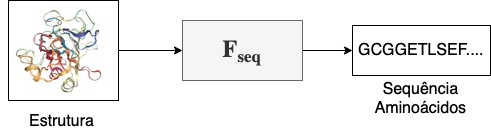
\includegraphics[width=.8\textwidth]{figuras/metodologia-SeqDes.jpg}
  \caption{O projeto de sequências se resume a desenvolver uma 
           função $F_{seq}$ que mapeia uma estrutura proteica tridimensional em uma sequência de aminoácidos.}
\end{figure}

\subsection{Baseado em Busca}

No projeto de sequências baseado em busca, 
a função $F_{seq}$ é definida por um processo iterativo 
composto por etapas bem estruturadas.
Inicialmente, é gerada uma sequência de aminoácidos baseada em uma heurística inicial $H$. 
A sequência resultante é avaliada por uma função objetivo $F_{obj}$, 
que calcula a métrica a ser otimizada. 
Se a sequência atual for melhor que a sequência anterior de acordo com a métrica definida, 
o Agente $A$ a adota como nova sequência final e realiza mutações na sequência atual. 
Esse processo é repetido até que um critério de parada seja atingido, 
como um número máximo de iterações ou a convergência em $F_{obj}$.


\begin{figure}[H]
  \centering
  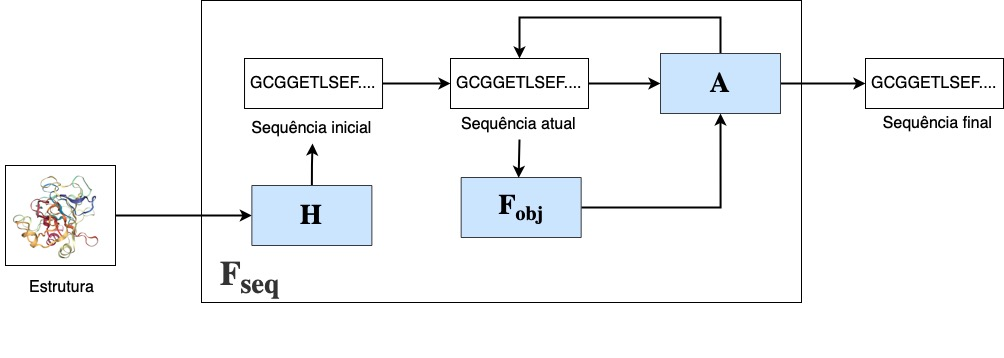
\includegraphics[width=.8\textwidth]{figuras/metodologia-SearchBased.jpg}
  \caption{O projeto de sequências baseado em busca define $F_{seq}$ como um processo iterativo que combina uma 
           heurística inicial $H$, a avaliação por $F_{obj}$ e as modificações realizadas pelo Agente $A$. O processo é repetido até atingir um limiar calculado por $F_{obj}$.}
  \label{fig:seqdes_search_based}
\end{figure}

O \textit{Rosetta} \cite{Rosetta} se baseia em um pipeline como este, 
no qual a heurística inicial $H$ utiliza a sequência de uma proteína
estruturalmente semelhante como ponto de partida. 
A função objetivo $F_{obj}$ avalia a energia livre da proteína,
considerando fatores como interações de Van der Waals,
interações eletrostáticas e ligações de hidrogênio.
O Agente $A$ utiliza o Método de Monte Carlo (MMC) para realizar mutações
e adotar configurações com menor energia livre.
Abordagens alternativas podem usar a similaridade estrutural como função objetivo,
sendo uma métrica amplamente utilizada o \textit{Template Modeling Score} (TMScore) \cite{tmscore}.

\subsection{Baseado em Aprendizado Profundo}

O projeto de sequências baseado em aprendizado profundo define a função $F_{seq}$ 
a partir de redes neurais artificiais. 
O \cite{ProteinMPNN} por exemplo, 
determina a $F_{seq}$ como uma rede neural profunda, denominada \textit{ProteinMPNN}, 
que mapeia de forma direta a estrutura alvo à sequência de aminoácidos. 
A rede é construída através de uma \textit{Message Passing Neural Network} (MPNN) 
composta por uma arquitetura \textit{encoder-decoder} 
que se baseia nas características da estrutura como distância e orientação dos átomos no espaço, 
para fazer predições \cite{ProteinMPNN}. 

\begin{figure}[H]
  \centering
  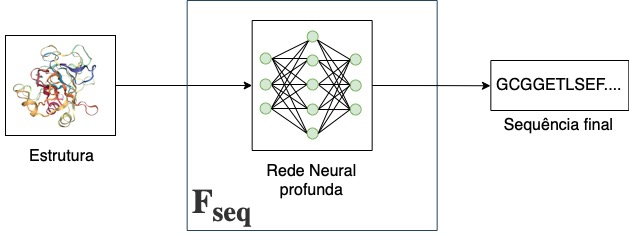
\includegraphics[width=.8\textwidth]{figuras/metodologia-DeepLearningBased.jpg}
  \caption{Projeto de Sequências baseado em aprendizado profundo.}
\end{figure}

\section{Proposta}
\label{section:Proposta}

Além de suscitar uma possível resposta imunológica, 
o tratamento da hemofilia tipo B baseado na infusão de fator IX
é custoso devido ao pouco tempo de vida da proteína na corrente sanguínea, demandando infusões frequentes. 
Neste sentido, este trabalho busca responder à seguinte pergunta científica: 
É possível, através de projeto de sequências, projetar uma proteína que desempenhe a mesma função do fator IX, 
mas com maior estabilidade, menor imunogenicidade e menos necessidade de infusões?

Para responder a esta questão, formulamos a hipótese de que, 
se existir uma proteína alternativa superior ao Fator IX, 
ela deverá ser estruturalmente similar. 
Assim, o objetivo será identificar proteínas estruturalmente semelhantes que atendam aos critérios estabelecidos.
Para simplificar o problema, focaremos no projeto do domínio protease, 
reconhecido como o mais relevante para a função do fator IX.

Nossa proposta consiste no desenvolvimento de um \textit{pipeline} que combina estratégias de busca 
com aprendizado profundo para otimização de sequências proteicas. 
Esse \textit{pipeline} será estruturado em três módulos principais: Condições Iniciais, 
Treinamento e Geração de Sequências.






O módulo de Condições Iniciais tem como objetivo obter a sequência inicial de aminoácidos 
por meio da heurística \( H \), além de calcular o erro inicial associado a essa sequência 
utilizando a função objetivo \( F_{\text{obj}} \). 
Para isso, empregaremos o \textit{ProteinMPNN} como heurística \( H \) 
e o TMScore como métrica de avaliação estrutural \( F_{\text{obj}} \).  

Diferente do uso de agentes que realizam mutações aleatórias, como no \textit{Rosetta},
no módulo de Treinamento treinaremos uma rede neural profunda, o \textit{GenSeq}, para atuar como o Agente $A$,
sendo capaz de realizar mutações que otimizem a similaridade com a estrutura alvo, isto é, o Fator IX.

Por fim, no módulo de Geração de Sequências, 
o agente treinado será utilizado para produzir um conjunto variantes proteicas estruturalmente semelhantes ao Fator IX,
por meio de um processo de mutação orientado. 
As sequências geradas serão então avaliadas para identificar possíveis candidatas viáveis 
que possam substituir o Fator IX no tratamento da hemofilia tipo B.



\begin{figure}[H]
  \centering
  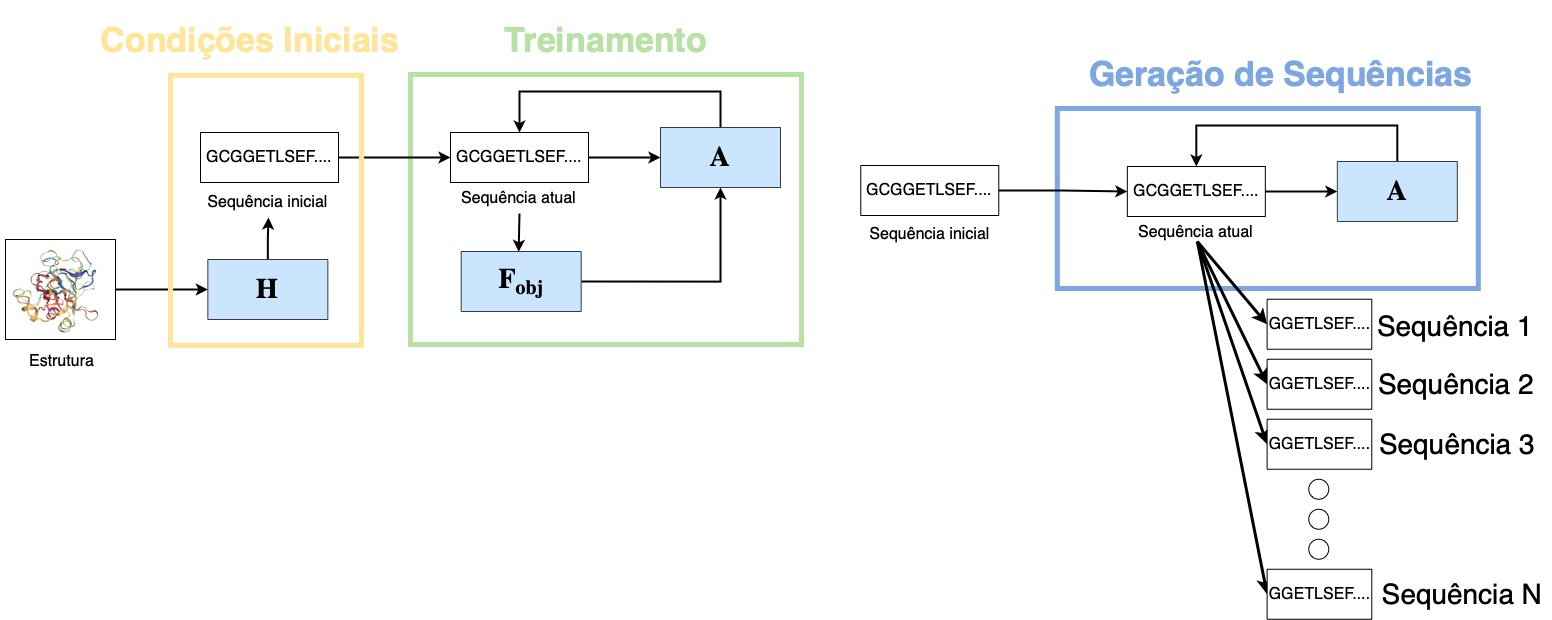
\includegraphics[width=.8\textwidth]{figuras/metodologia-pipeline_proposta.jpg}
  \caption{Pipeline proposto para o projeto de sequências.}
  \label{fig:proposta}
\end{figure}

\section{Objetivos}

\begin{enumerate}
  \item Obter um conjunto de sequências de aminoácidos que mimetizem a estrutura do fator de coagulação IX baseado na métrica TMScore.
  \item Avaliar, dentro do conjunto de proteínas obtidas em 1, quais possuem potencial de substituir o Fator IX de modo tornar o tratamento de Hemofilia tipo B mais acessível e eficiente.
  \item Desenvolver um \textit{pipeline} genérico que produza sequências que mimetizem uma estrutura qualquer.
\end{enumerate}
